\documentclass[conference]{IEEEtran}
\usepackage[utf8]{inputenc}
\usepackage{amsmath}
\usepackage{amsfonts}
\usepackage{amssymb}
\usepackage{graphicx}
\usepackage[left=1cm, right=1cm, top=1cm, bottom=1cm]{geometry}
\usepackage{float} % For [H] placement of figures
\usepackage{hyperref} % For clickable links and references
\usepackage{listings} % For code snippets
\usepackage{xcolor} % For coloring code

\title{Hybrid AI for Intelligent Street Lighting: Regression, Fuzzy Reasoning, and Evolutionary Tuning}
\author{
\IEEEauthorblockN{Everyone has done equal amount of work :)\\
Michał Mazurek, Marcin Basisty, Łukasz Święch, Byeongjun Min}
\IEEEauthorblockA{
Faculty of Physics and Applied Computer Science\\
AGH University of Science\\
Krakow, Poland\\
}
}

\begin{document}

\maketitle
\begin{abstract}
Urban street lighting plays a critical role in ensuring safety, mobility, and quality of life, yet it is also a major contributor to municipal energy consumption. Traditional lighting systems are typically static or reactive, leading to unnecessary energy use and sometimes inadequate illumination in dynamic urban environments. The challenge is to design a control system that intelligently adapts to fluctuating pedestrian activity, traffic patterns, and environmental conditions while balancing energy efficiency and public safety.

This report presents a hybrid artificial intelligence framework that addresses this challenge by combining predictive modeling, interpretable reasoning, and evolutionary optimization. A data-driven regression model forecasts short-term lighting demand using heterogeneous sensor and contextual inputs, including ambient light, occupancy, traffic density, and temporal indicators. These predictions are further refined through a fuzzy-rule-based expert layer, embedding safety-aware logic that ensures sufficient illumination under uncertain or extreme conditions.

To optimize system performance, fuzzy membership functions and control thresholds are tuned using a multi-objective evolutionary algorithm, producing a Pareto-optimal set of solutions that balance energy savings and predicted safety risk. Experimental evaluation with realistic urban datasets shows that the hybrid approach achieves substantial energy reduction while maintaining safety and interpretability, outperforming purely data-driven or static strategies.

By integrating predictive intelligence, rule-based reasoning, and optimization, this work provides a robust, adaptive, and transparent solution for modern smart city lighting. It demonstrates how hybrid AI can transform urban infrastructure, enabling sustainable, safe, and context-aware illumination.
\end{abstract}

\section{Introduction}
Public street lighting is a critical component of urban infrastructure, directly affecting road safety, pedestrian security, and quality of life. Conventional lighting systems rely on static schedules or simple threshold-based rules, which often lead to excessive energy consumption during periods of low demand. As cities pursue sustainability goals and operational cost reductions, there is a growing need for adaptive lighting systems that respond dynamically to real-world conditions.

Recent advances in sensing, communication, and Internet of Things (IoT) technologies have enabled smart lighting infrastructures capable of collecting rich, high-dimensional data. These data streams include ambient light levels, weather conditions, pedestrian and traffic activity, and historical energy usage. While such data enable intelligent control, they also introduce complexity and uncertainty that challenge traditional rule-based systems.

Machine learning (ML) techniques are well suited to modeling nonlinear relationships between environmental conditions, human activity, and lighting demand. However, purely data-driven approaches often lack interpretability and may exhibit unstable behavior under noisy or unseen conditions. In safety-critical public infrastructure, this opacity limits trust, accountability, and deployability.

Hybrid AI approaches that combine ML with classical artificial intelligence techniques offer a promising solution. In particular, fuzzy logic systems provide interpretable, human-readable decision rules that can enforce conservative behavior under uncertainty. When integrated with ML predictions, fuzzy reasoning can stabilize outputs and incorporate domain knowledge explicitly.

This work proposes a hybrid smart street lighting control framework that integrates ML-based demand estimation, fuzzy-rule-based reasoning, and evolutionary optimization. The following sections describe the dataset, modeling methodology, fuzzy control design, optimization strategy, evaluation protocol, and experimental results.

\subsection{Dataset Description and Preprocessing}
The experiments are conducted using the IoT-enabled smart lighting dataset from Kaggle \cite{smartlighting_dataset}. The dataset contains sensor measurements collected from multiple urban zones, capturing environmental, occupancy, and energy-related features relevant to adaptive street lighting. Key features include:

\begin{itemize}
    \item \texttt{ambient\_light\_lux}: measured light level (lux)
    \item \texttt{temperature\_celsius}: ambient temperature
    \item \texttt{motion\_detected}: binary motion sensor
    \item \texttt{occupancy\_count}: number of detected people
    \item \texttt{traffic\_density}: estimated traffic level
    \item \texttt{avg\_pedestrian\_speed}: average pedestrian speed
    \item \texttt{weather\_condition}: categorical weather indicators (foggy, cloudy, rainy, etc.)
    \item \texttt{special\_event\_flag}: indicator for concerts, events, etc.
    \item \texttt{energy\_price\_per\_kwh}: cost of electricity
    \item \texttt{prev\_hour\_energy\_usage\_kwh}: past energy usage
    \item \texttt{adjusted\_light\_intensity}: target lighting output (\%)
\end{itemize}

Categorical variables, including weather conditions and zone identifiers, are transformed using one-hot encoding. All numerical features are standardized using z-score normalization to ensure comparable scales across inputs. The dataset is then split into training and testing subsets to support unbiased evaluation of predictive performance.

The target variable for supervised learning is the adjusted lighting output, represented by \texttt{adjusted\_light\_intensity}, which reflects the effective lighting level selected under the given conditions.

\subsection{Safety Risk Score Calculation}
To explicitly incorporate safety considerations into the lighting control framework, a composite safety risk score was computed for each observation. This score quantifies the perceived risk level associated with pedestrian presence, traffic activity, and contextual events, and serves as an additional high-level feature for downstream decision-making.

The risk score is derived from a weighted combination of normalized activity-related variables and binary contextual indicators. Specifically, the following features were selected due to their direct relevance to public safety in street lighting scenarios: pedestrian occupancy count, traffic density, average pedestrian speed, motion detection, and the presence of special events.

First, continuous variables—namely \texttt{occupancy\_count}, \texttt{traffic\_density}, and \texttt{avg\_pedestrian\_speed}—were normalized to the range $[0,1]$ using Min--Max scaling. This ensures comparable magnitudes across heterogeneous features and prevents dominance by variables with larger numerical ranges. The binary \texttt{motion\_detected} indicator was retained in its original form.

A base safety risk score was then computed as a weighted linear combination of these components:
\begin{equation}
R_{\text{base}} = 0.15 \cdot M + 0.35 \cdot O + 0.35 \cdot T + 0.15 \cdot S
\end{equation}
where $M$ denotes motion detection, $O$ represents normalized occupancy count, $T$ corresponds to normalized traffic density, and $S$ denotes normalized pedestrian speed. The weights were selected heuristically to reflect the relative importance of each factor, with greater emphasis placed on real-time motion detection and crowd presence.

To account for atypical conditions associated with concerts, public gatherings, or other special events, an amplification factor was applied when the binary \texttt{special\_event\_flag} was active. The final safety risk score was computed as:
\begin{equation}
R_{\text{safety}} = R_{\text{base}} \cdot \left(1 + \alpha \cdot E \right)
\end{equation}
where $E \in \{0,1\}$ indicates the occurrence of a special event and $\alpha = 0.30$ controls the degree of risk amplification. This formulation increases sensitivity to situations that typically involve elevated pedestrian density and safety concerns.

Finally, the resulting safety risk score was clipped to the interval $[0,1]$ to ensure numerical stability and interpretability. The computed score was appended to the feature set as \texttt{safety\_risk\_score} and used to support safety-aware control decisions in subsequent modeling stages.

\subsection{Feature Skewness and Transformation}

Exploratory analysis revealed that some numerical features exhibit high positive skewness, particularly \texttt{ambient\_light\_lux} and \texttt{occupancy\_count}. To mitigate the effect of skewed distributions on regression models, the log transformation $\log1p(x)$ was applied to these features:

\begin{figure}[H]
    \centering
    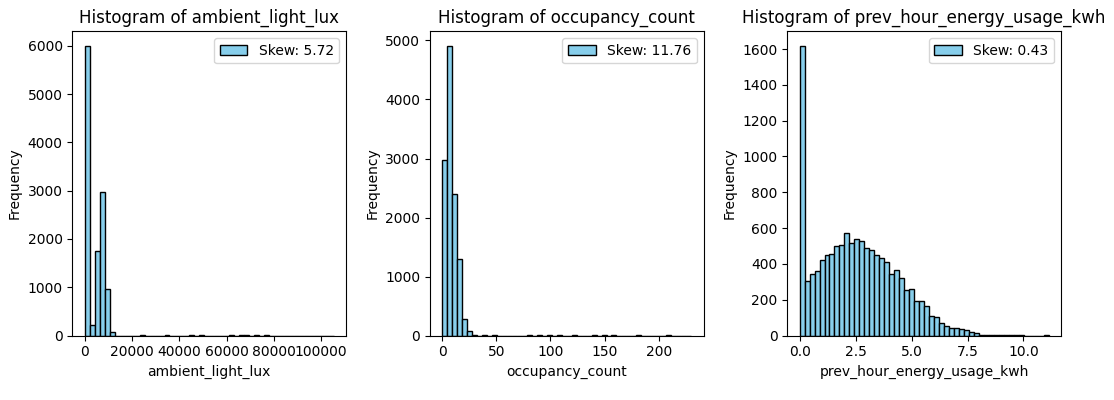
\includegraphics[width=\linewidth]{assets/SkewedFeatures.png}
    \caption{Features tested for skewness.}
    \label{fig:placeholder}
\end{figure}

\begin{equation}
x' = \log(1 + x)
\end{equation}

This transformation improves linearity and reduces the influence of extreme values, helping the machine learning predictor to converge more effectively.

\begin{figure}[H]
    \centering
    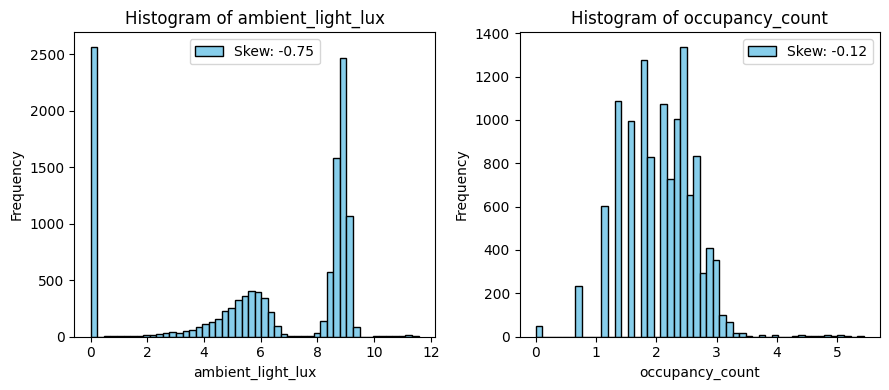
\includegraphics[width=\linewidth]{assets/LessSkewedFeatures.png}
    \caption{Features after reducing the skewness.}
    \label{fig:placeholder}
\end{figure}

\subsection{Machine Learning-Based Lighting Demand Estimation}

A supervised machine learning model is trained to learn the mapping from the preprocessed input features to the target lighting intensity. The ML predictor captures nonlinear relationships between environmental conditions, human activity, and lighting demand. By learning from historical data, the model implicitly encodes temporal and contextual patterns such as increased illumination requirements during high occupancy, adverse weather, or special events.

The predicted lighting intensity serves as an intermediate decision signal rather than a final control action. This design allows subsequent reasoning layers to refine or constrain the ML output based on explicit safety and operational rules.

\section{Evaluation Protocol}
The proposed system is evaluated by comparing three control strategies: a static baseline, an ML-only controller, and the hybrid ML + Fuzzy controller. Since the target variable (\texttt{adjusted\_light\_intensity}) is continuous, performance is quantified using regression metrics:

\begin{itemize}
    \item \textbf{Root Mean Absolute Error (RMAE)}: measures the average magnitude of prediction errors in the same units as the target, providing an interpretable estimate of typical deviation.
    \item \textbf{Mean Absolute Error (MAE)}: quantifies the mean absolute difference between predicted and actual lighting intensity across the test set.
    \item \textbf{Coefficient of Determination ($R^2$)}: indicates the proportion of variance in the target variable explained by the model, capturing overall goodness of fit.
\end{itemize}

To rigorously compare model performance, the paired Wilcoxon signed-rank test is applied to per-run prediction errors. This non-parametric test assesses whether differences in performance are statistically significant without assuming normality:

\begin{itemize}
    \item Compute the paired differences in prediction error (MAE or RMAE) for each test instance between two models.
    \item Apply the Wilcoxon signed-rank test to obtain the test statistic and associated $p$-value.
    \item If $p < 0.05$, the performance difference is considered significant.
\end{itemize}

Combining regression metrics with statistical testing allows both quantitative and inferential evaluation. Models can be ranked based on median error reduction and statistical significance, providing confidence that observed improvements—such as those achieved by the hybrid ML + Fuzzy controller over the ML-only model—are meaningful and not due to chance. This multi-metric evaluation ensures that gains in accuracy do not come at the expense of unrealistic or unstable control outputs, while also supporting operational robustness and safety compliance.

\section{Fuzzy Logic System for Adaptive Lighting Control}

\subsection{Motivation and Overview}
To enhance the adaptability and interpretability of the lighting control system, a fuzzy logic approach was implemented alongside the Multi-Layer Perceptron (MLP) model. The primary motivation was to introduce human-like reasoning into the decision-making process for adjusting light intensity, particularly in situations where the MLP's predictions might deviate significantly from expected behavior or when environmental factors necessitate a more robust, rule-based adjustment. The fuzzy system provides interpretable rules based on environmental conditions and estimated activity levels, allowing for a transparent modification of the MLP's raw output.

\subsection{Fuzzy Variables and Membership Functions}
The fuzzy inference system was designed with two input (antecedent) variables and one output (consequent) variable, all normalized to the interval $[0,1]$:

\begin{itemize}
    \item \textbf{Activity Level}: Represents the estimated human or vehicular presence in the lighting zone. This variable is derived from \texttt{occupancy\_count} and normalized such that higher values indicate increased activity. Triangular membership functions (\texttt{fuzz.trimf}) were defined for the linguistic terms \emph{low}, \emph{medium}, and \emph{high}.
    
    \item \textbf{Visibility Level}: Reflects environmental conditions affecting visibility. This is computed as a composite score based on \texttt{ambient\_light\_lux}, \texttt{weather\_condition} (Foggy, Rainy, Cloudy), and the hour of the day. A dedicated function, \texttt{compute\_visibility\_score\_weighted}, combines these factors while assigning greater weight to ambient light and day/night conditions. Membership functions were defined for \emph{poor}, \emph{normal}, and \emph{good} visibility.
    
    \item \textbf{Lighting Intensity}: The output variable representing the recommended adjusted light intensity. Membership functions were defined for the linguistic terms \emph{dim}, \emph{normal}, and \emph{full}.
\end{itemize}

The \texttt{scikit-fuzzy} (\texttt{skfuzzy}) library was used to define the fuzzy sets and their corresponding triangular membership functions, as implemented in the notebook cells defining the \texttt{build\_fuzzy\_system()} function.

\subsection{Fuzzy Rule Base}
The rule base constitutes the core of the fuzzy logic system and encodes expert knowledge for lighting adjustment based on activity and visibility conditions. A total of nine rules were defined to cover all relevant combinations:

\begin{enumerate}
    \item IF activity is \emph{high}, THEN lighting is \emph{full}.
    \item IF activity is \emph{medium} AND visibility is \emph{poor}, THEN lighting is \emph{full}.
    \item IF activity is \emph{medium} AND visibility is \emph{normal}, THEN lighting is \emph{normal}.
    \item IF activity is \emph{low} AND visibility is \emph{good}, THEN lighting is \emph{dim}.
    \item IF activity is \emph{low} AND visibility is \emph{poor}, THEN lighting is \emph{normal}.
    \item IF activity is \emph{low} AND visibility is \emph{normal}, THEN lighting is \emph{dim}.
    \item IF activity is \emph{medium} AND visibility is \emph{good}, THEN lighting is \emph{normal}.
    \item IF activity is \emph{high} AND visibility is \emph{good}, THEN lighting is \emph{full}.
    \item IF activity is \emph{high} AND visibility is \emph{poor}, THEN lighting is \emph{full}.
\end{enumerate}

These rules are evaluated using a Mamdani-style fuzzy inference mechanism, and the aggregated fuzzy output is defuzzified to obtain a crisp lighting intensity value.

\subsection{Integration with MLP Predictions}

The fuzzy logic system acts as a correctional layer over the MLP predictions. The integration process consists of the following steps:

\begin{enumerate}
    \item \textbf{Independent Prediction}: The MLP model, \texttt{mlp\_model}, generates a baseline prediction of the adjusted lighting intensity, denoted as $\hat{y}_{\text{MLP}}^{\text{test}}$. In parallel, the fuzzy inference system computes its own prediction, $\hat{y}_{\text{Fuzzy}}^{\text{test}}$, using the \texttt{fuzzy\_predict\_target\_daynight} function. This function includes a calibration step based on training data to align fuzzy outputs with the target scale.
    
    \item \textbf{Deviation Calculation}: The absolute deviation between the MLP and fuzzy predictions on the training set, $\Delta_{\text{train}}$, is used to compute a deviation threshold, typically defined as the 90th percentile. This threshold identifies cases where the MLP output diverges significantly from the fuzzy system recommendation.
    
    \item \textbf{Weighted Correction}: For test samples, if the deviation $\Delta_{\text{test}}$ exceeds the predefined threshold, the fuzzy system output is used to correct the MLP prediction. A weighting function, \texttt{correct\_mlp\_with\_fuzzy}, blends the two predictions smoothly based on the deviation magnitude and a maximum weighting factor $w_{\max}$. This ensures that fuzzy intervention occurs only when meaningful disagreement is detected.
\end{enumerate}

\subsection{Optimization of Fuzzy Rules}

Initial attempts were made to optimize fuzzy rule thresholds and system parameters, including \texttt{ambient\_dark}, \texttt{ambient\_dim}, \texttt{ambient\_bright}, \texttt{activity\_low}, \texttt{activity\_medium}, $\alpha$, and \texttt{max\_delta}, using the Optuna framework. Both \texttt{HyperbandPruner} and \texttt{TPESampler} were explored to search the parameter space efficiently.

\subsection{Performance Enhancement}

The hybrid MLP+Fuzzy model demonstrated improved robustness, particularly in handling outlier cases where the standalone MLP predictions deviated substantially. The fuzzy correction mechanism contributed to reductions in RMSE and MAE, as well as a slight improvement in $R^2$ on the test set. These results highlight the effectiveness of combining data-driven learning models with interpretable, rule-based fuzzy systems for adaptive lighting control.

\section{Multi-Objective Differential Evolution with Sobol Initialization}

This study employs a multi-objective Differential Evolution (DE) algorithm to optimize lighting control strategies under competing objectives. The algorithm minimizes energy consumption while simultaneously reducing predicted safety violations estimated by a learned model. To enhance search efficiency and population diversity, Sobol quasi-random sampling is used for population initialization.

\subsubsection{Population Initialization}

The initial population is generated using Sobol low-discrepancy sequences, which provide a more uniform coverage of the decision space than purely random sampling. Given lower and upper bounds $\mathbf{l}, \mathbf{u} \in \mathbb{R}^D$ for a $D$-dimensional decision vector, the Sobol samples are scaled as
\begin{equation}
\mathbf{x}_i = \mathbf{l} + (\mathbf{u} - \mathbf{l}) \odot \mathbf{s}_i,
\end{equation}
where $\mathbf{s}_i \in [0,1]^D$ denotes the Sobol sample and $\odot$ represents element-wise multiplication.

\subsubsection{Multi-Objective Fitness Function}

Each candidate solution $\mathbf{x}$ represents lighting intensity levels across discrete time blocks. The optimization problem is formulated as a bi-objective minimization:
\begin{equation}
\min_{\mathbf{x}} \; \mathbf{f}(\mathbf{x}) = \left( f_1(\mathbf{x}), f_2(\mathbf{x}) \right).
\end{equation}

\paragraph{Objective 1: Average Energy Consumption}

The average energy consumption is computed as
\begin{equation}
f_1(\mathbf{x}) = \frac{1}{N} \sum_{i=1}^{N} P_{\max} \cdot \frac{x_{h_i}}{100} \cdot \Delta t_i,
\end{equation}
where $P_{\max}$ is the maximum lighting power of a zone, $x_{h_i}$ denotes the lighting intensity assigned to hour block $h_i$, $\Delta t_i$ is the duration of the $i$-th evaluation interval, and $N$ is the total number of evaluation samples.

\paragraph{Objective 2: Predicted Safety Violation}

The second objective minimizes the expected safety violation predicted by a trained multilayer perceptron (MLP):
\begin{equation}
f_2(\mathbf{x}) = \frac{1}{N} \sum_{i=1}^{N} \hat{v}_i(\mathbf{x}),
\end{equation}
where $\hat{v}_i(\mathbf{x})$ is the MLP-predicted violation score for the $i$-th evaluation instance given decision vector $\mathbf{x}$. Model inference is performed in evaluation mode without gradient computation.

\subsubsection{Differential Evolution Operators}

The algorithm adopts the DE/rand/1/bin strategy.

\paragraph{Mutation}

For each target vector $\mathbf{x}_i$, three distinct vectors $\mathbf{x}_{r_1}$, $\mathbf{x}_{r_2}$, and $\mathbf{x}_{r_3}$ are randomly selected from the population. A mutant vector is generated as
\begin{equation}
\mathbf{v}_i = \mathbf{x}_{r_1} + F \cdot (\mathbf{x}_{r_2} - \mathbf{x}_{r_3}),
\end{equation}
where $F \in (0,1]$ is the mutation factor. Boundary constraints are enforced via clipping:
\begin{equation}
\mathbf{v}_i \leftarrow \min\left(\max(\mathbf{v}_i, \mathbf{l}), \mathbf{u}\right).
\end{equation}

\paragraph{Crossover}

Binomial crossover is applied to generate the trial vector $\mathbf{u}_i$:
\begin{equation}
u_{i,j} =
\begin{cases}
v_{i,j}, & \text{if } r_j < CR \text{ or } j = j_{\text{rand}}, \\
x_{i,j}, & \text{otherwise},
\end{cases}
\end{equation}
where $CR \in [0,1]$ is the crossover rate, $r_j \sim \mathcal{U}(0,1)$, and $j_{\text{rand}}$ ensures that at least one component is inherited from the mutant vector.

\paragraph{Selection via Pareto Dominance}

Selection is governed by Pareto dominance. A trial vector $\mathbf{u}_i$ replaces the current vector $\mathbf{x}_i$ if
\begin{equation}
\mathbf{f}(\mathbf{u}_i) \preceq \mathbf{f}(\mathbf{x}_i)
\quad \text{and} \quad
\mathbf{f}(\mathbf{u}_i) \neq \mathbf{f}(\mathbf{x}_i),
\end{equation}
where $\preceq$ denotes component-wise inequality. This ensures that the trial solution is no worse in all objectives and strictly better in at least one objective.

\subsubsection{Pareto Front Extraction}

After a fixed number of generations, the final population is filtered to extract the set of non-dominated solutions:
\begin{equation}
\mathcal{P} = \left\{ \mathbf{x}_i \mid \nexists \mathbf{x}_j : \mathbf{f}(\mathbf{x}_j) \prec \mathbf{f}(\mathbf{x}_i) \right\},
\end{equation}
where $\prec$ denotes strict Pareto dominance. The resulting set $\mathcal{P}$ approximates the Pareto front.

\subsubsection{Outcome}

The extracted Pareto-optimal solutions characterize the trade-off between energy efficiency and safety performance. By integrating Sobol initialization with Pareto-based selection, the proposed approach achieves improved convergence robustness and maintains solution diversity relative to conventional randomly initialized or single-objective DE methods.


\section{Exploratory Data Analysis and Feature Relationships}
To better understand the structure of the dataset and the relationships between key features, several visualizations were created. These plots provide insight into patterns of energy consumption, pedestrian and traffic activity, environmental conditions, and safety considerations.

\subsection{Energy Consumption Patterns}
Mean hourly energy consumption was analyzed to identify temporal trends in street lighting demand. As expected, energy usage peaks during evening hours and decreases during low-activity periods, such as early morning. This pattern highlights the importance of adaptive control to reduce unnecessary energy expenditure during off-peak periods.

Energy consumption was also examined with respect to weather conditions. Results indicate that adverse conditions, such as rain or fog, lead to higher energy usage, reflecting increased lighting needs for visibility and safety.

\begin{figure}[H]
\centering
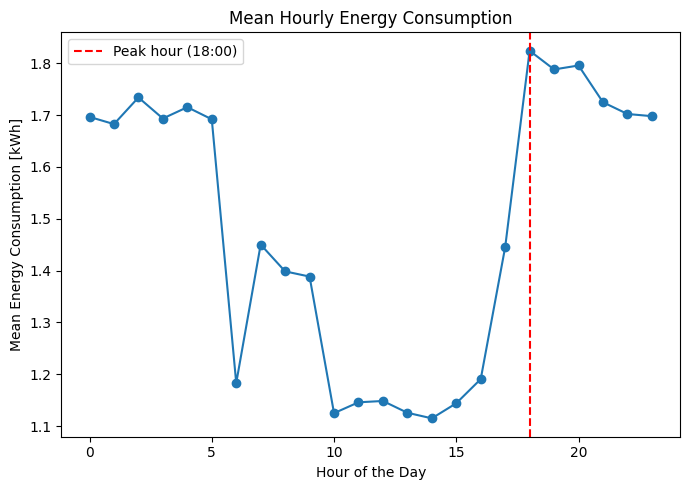
\includegraphics[width=0.6\linewidth]{assets/MeanHourlyConsumption.png}
\caption{Mean hourly energy consumption across a typical day, showing peak demand during evening hours and lower usage during early morning.}
\label{fig:mean_hourly_energy}
\end{figure}

\begin{figure}[H]
\centering
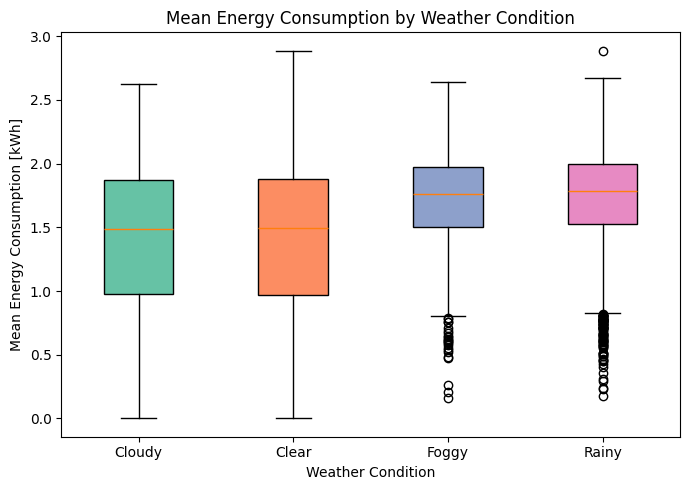
\includegraphics[width=0.6\linewidth]{assets/MeanEnergyByWeather.png}
\caption{Mean energy consumption by weather condition. Energy usage increases during adverse conditions such as rain or fog, reflecting higher lighting requirements for safety.}
\label{fig:energy_weather}
\end{figure}

\subsection{Traffic and Lighting Relationships}
The interaction between traffic density and lighting adjustments was explored. Mean light adjustments were observed to increase with higher traffic levels, demonstrating the system’s responsiveness to pedestrian and vehicle activity. Separate visualizations of light levels versus day/night periods confirmed that lighting demand is generally higher at night, with greater variability depending on traffic patterns.

Energy consumption was further analyzed against traffic density and temporal factors. During periods of high traffic density, energy usage increased noticeably, particularly during nighttime hours. Conversely, low-density periods corresponded to reduced lighting needs.

\begin{figure}[H]
\centering
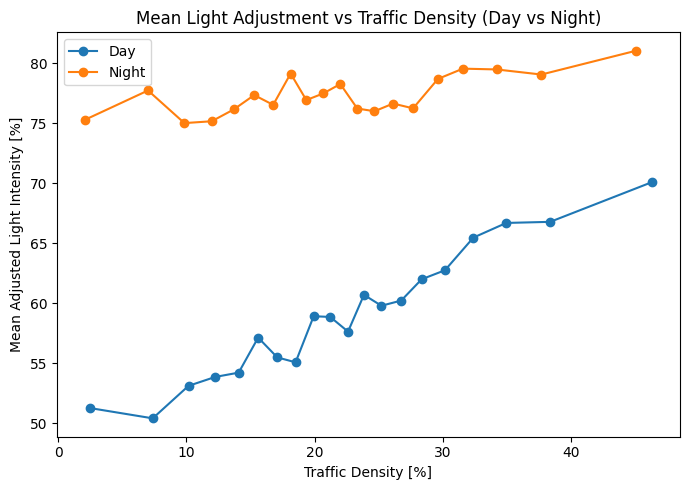
\includegraphics[width=0.6\linewidth]{assets/LightAdjustmentvsTrafficDensity.png}
\caption{Mean lighting adjustments versus traffic density, illustrating the system’s dynamic response to increasing pedestrian and vehicle activity.}
\label{fig:light_vs_traffic_density}
\end{figure}

\subsection{Safety and Special Events}
Energy usage was evaluated with respect to safety risk levels, showing that areas or periods with higher perceived risk were associated with increased lighting. This trend suggests that the system can prioritize safety through dynamic adjustments.

Additionally, mean energy consumption during special events was examined, revealing localized spikes in demand corresponding to increased pedestrian activity. This highlights the importance of incorporating contextual awareness in intelligent lighting control.

\begin{figure}[H]
\centering
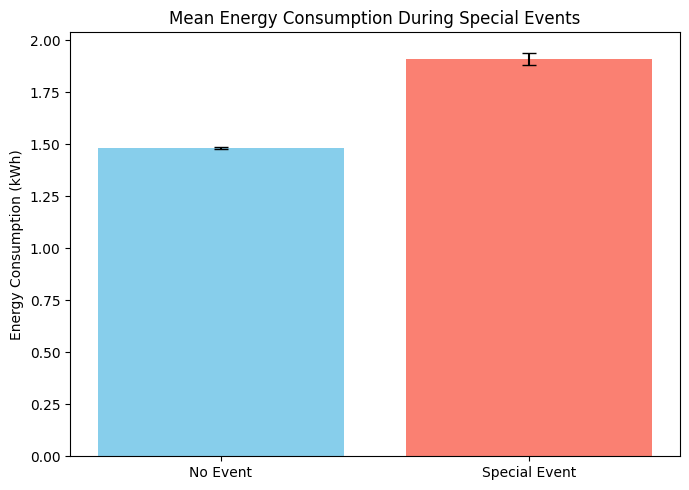
\includegraphics[width=0.6\linewidth]{assets/EnergySpecialEvent.png}
\caption{Mean energy consumption during special events, showing spikes in usage corresponding to increased pedestrian activity.}
\label{fig:energy_special_event}
\end{figure}

\begin{figure}[H]
\centering
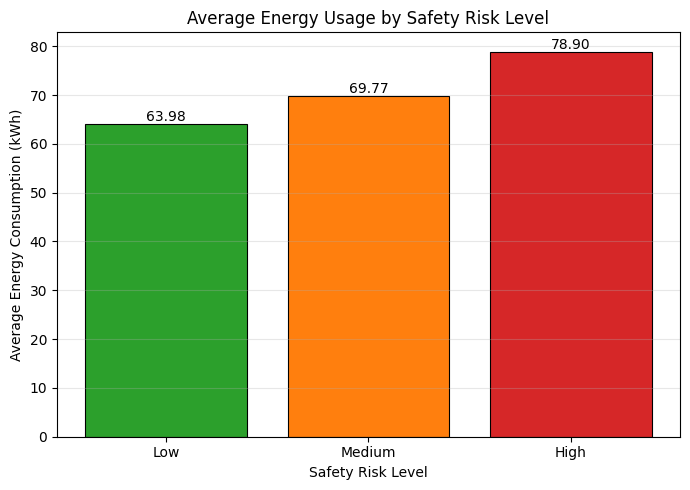
\includegraphics[width=0.5\linewidth]{assets/EnergyvsRisk.png}
\caption{Energy consumption by safety risk level, highlighting elevated lighting in higher-risk areas or periods to enhance visibility and safety.}
\label{fig:energy_vs_safety_risk}
\end{figure}

\subsection{Density-Level Analysis}
Finally, energy consumption was analyzed by density levels categorized as low, medium, and high. The results demonstrate a clear relationship between crowd or traffic density and lighting energy requirements, providing evidence that density-aware control strategies can further optimize energy efficiency without compromising safety.

\begin{figure}[H]
\centering
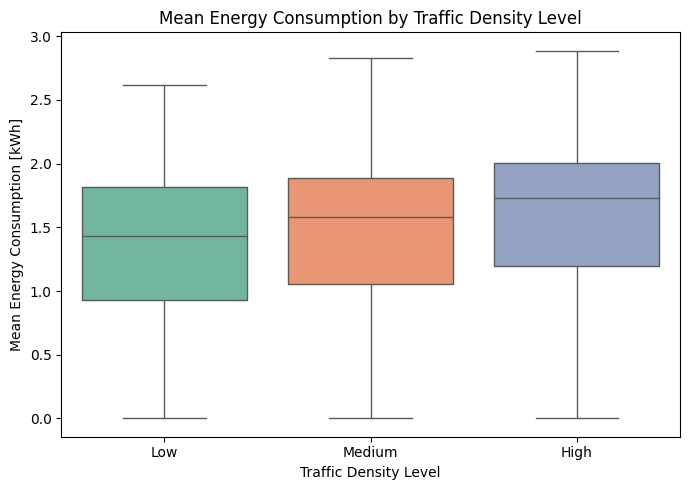
\includegraphics[width=0.6\linewidth]{assets/EnergyByTraffic.png}
\caption{Energy consumption across different traffic levels, showing increased usage during periods of higher pedestrian and vehicle activity.}
\label{fig:energy_by_traffic}
\end{figure}

\begin{figure}[H]
\centering
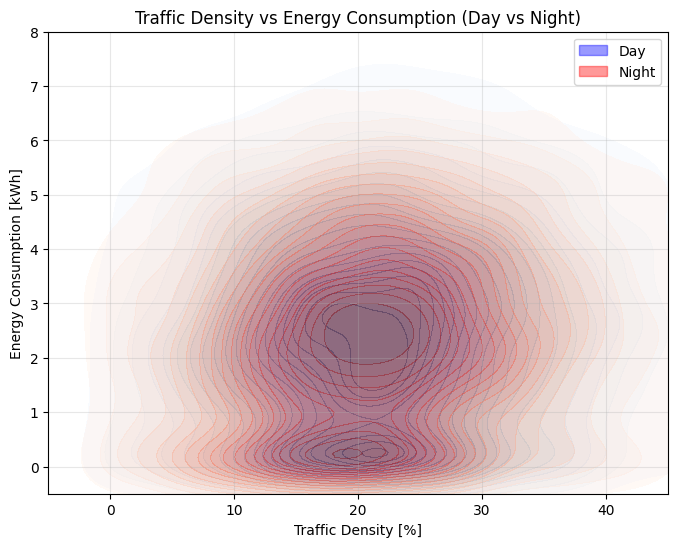
\includegraphics[width=0.6\linewidth]{assets/EnergyvsTrafficDensity.png}
\caption{Relationship between traffic density and energy consumption during day and night periods, highlighting higher energy demand at night with high traffic density.}
\label{fig:energy_vs_traffic_density}
\end{figure}

\subsection{Feature relationship analysis}
Below we included a few plots describing feature relationship within the dataset.

\begin{figure}[H]
\centering
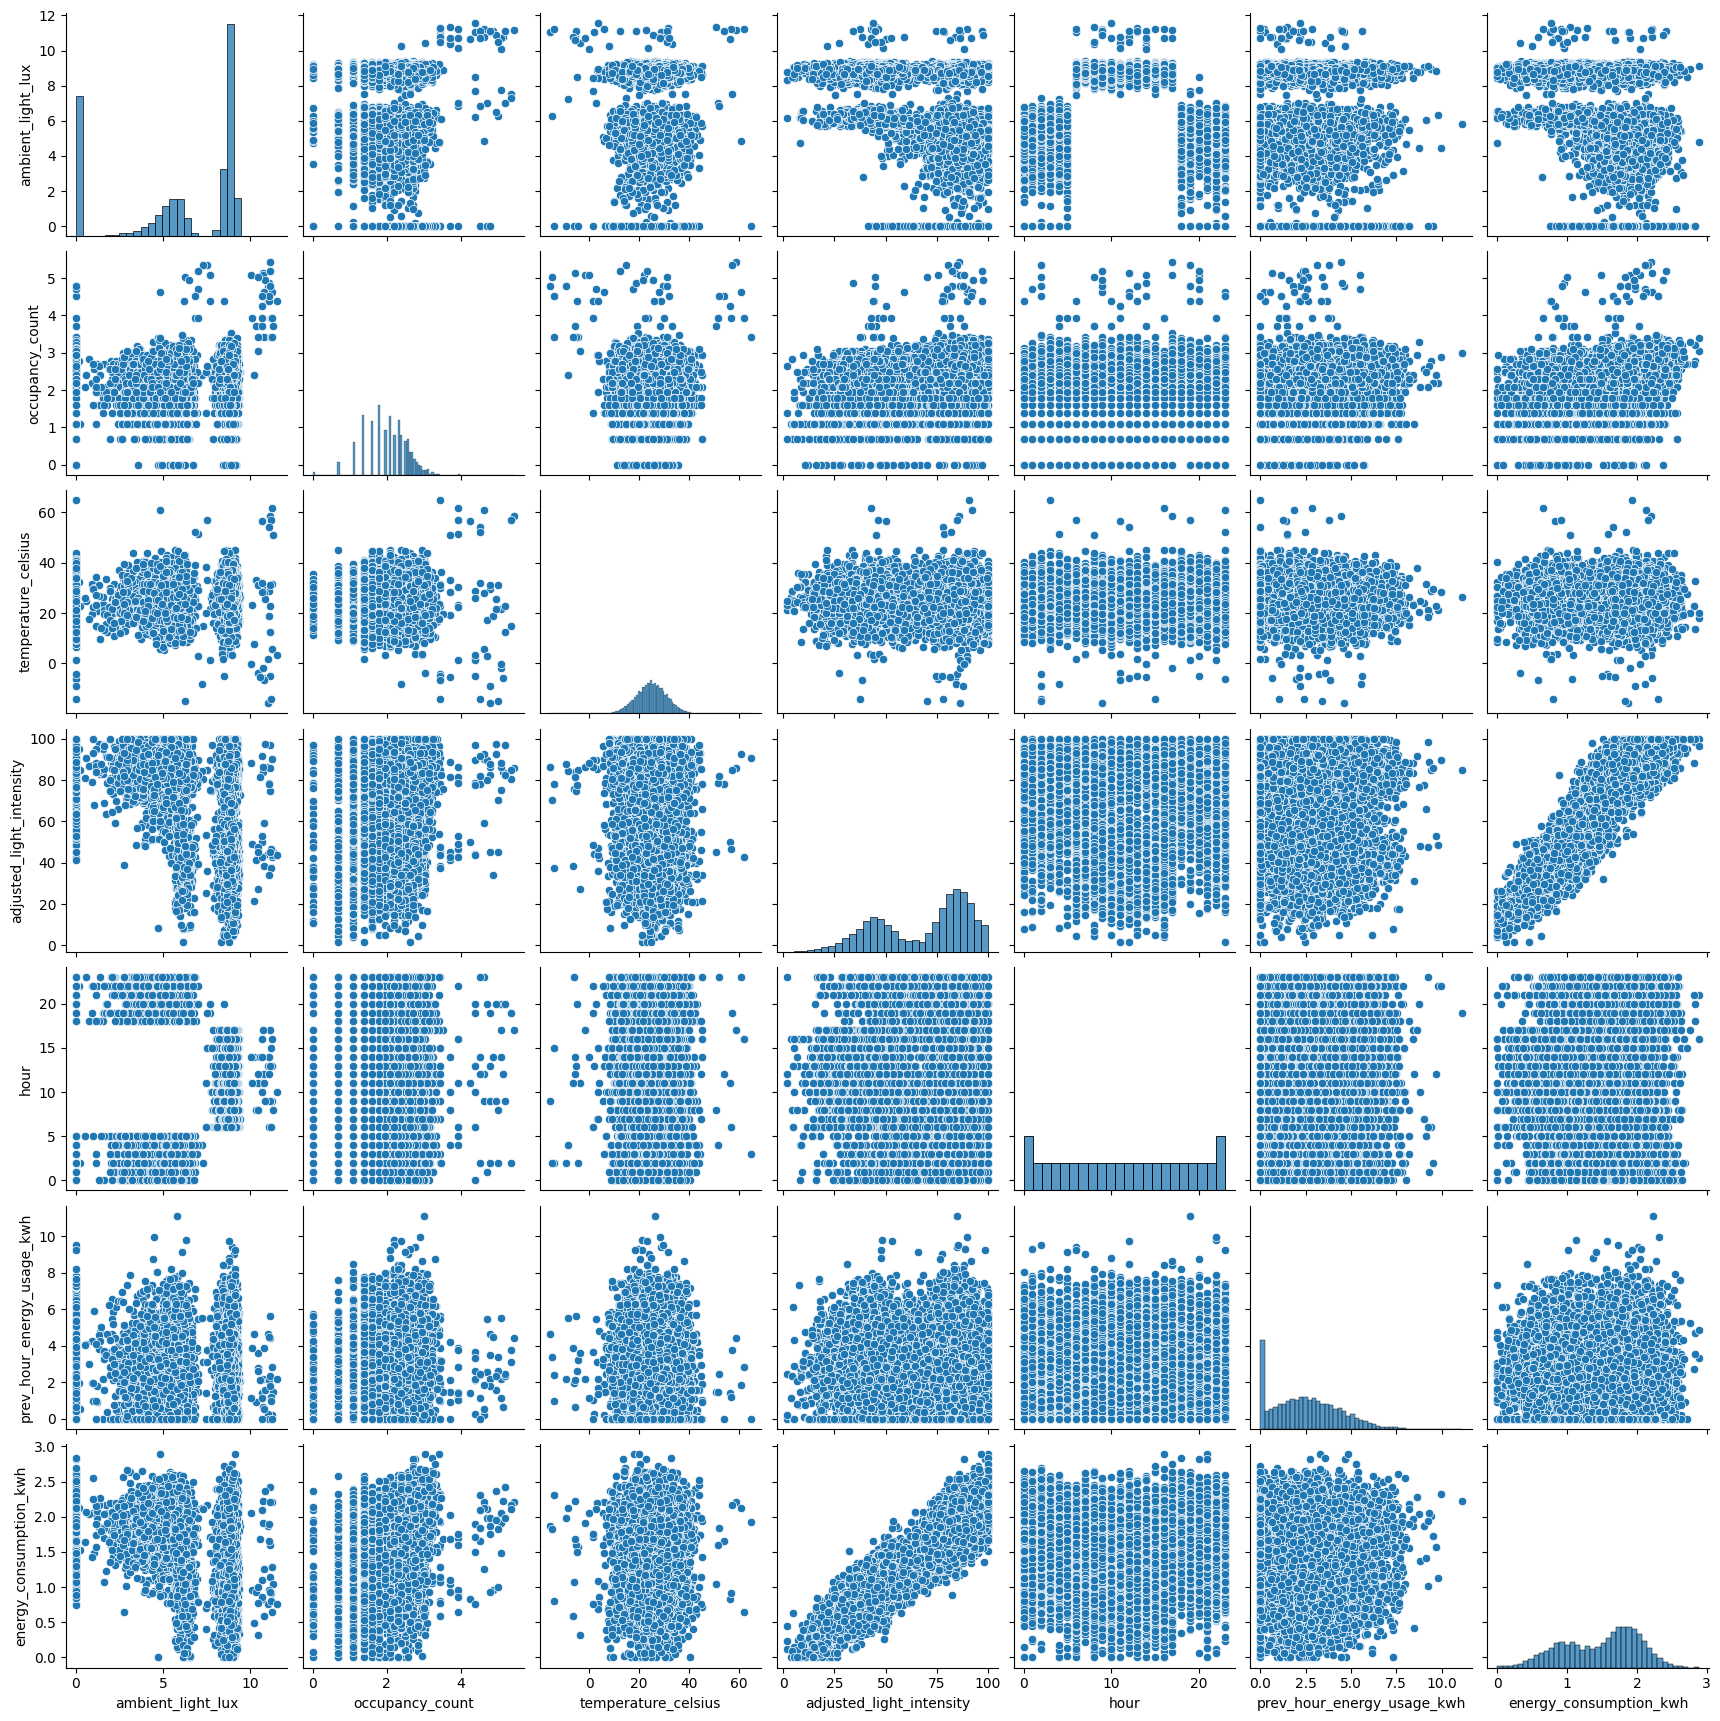
\includegraphics[width=0.4\textwidth]{assets/Pairplot.png}
\caption{Pairplot of selected features, visualizing pairwise relationships and distributions to identify correlations, nonlinear trends, and potential clusters.}
\label{fig:pairplot}
\end{figure}

\begin{figure}[H]
\centering
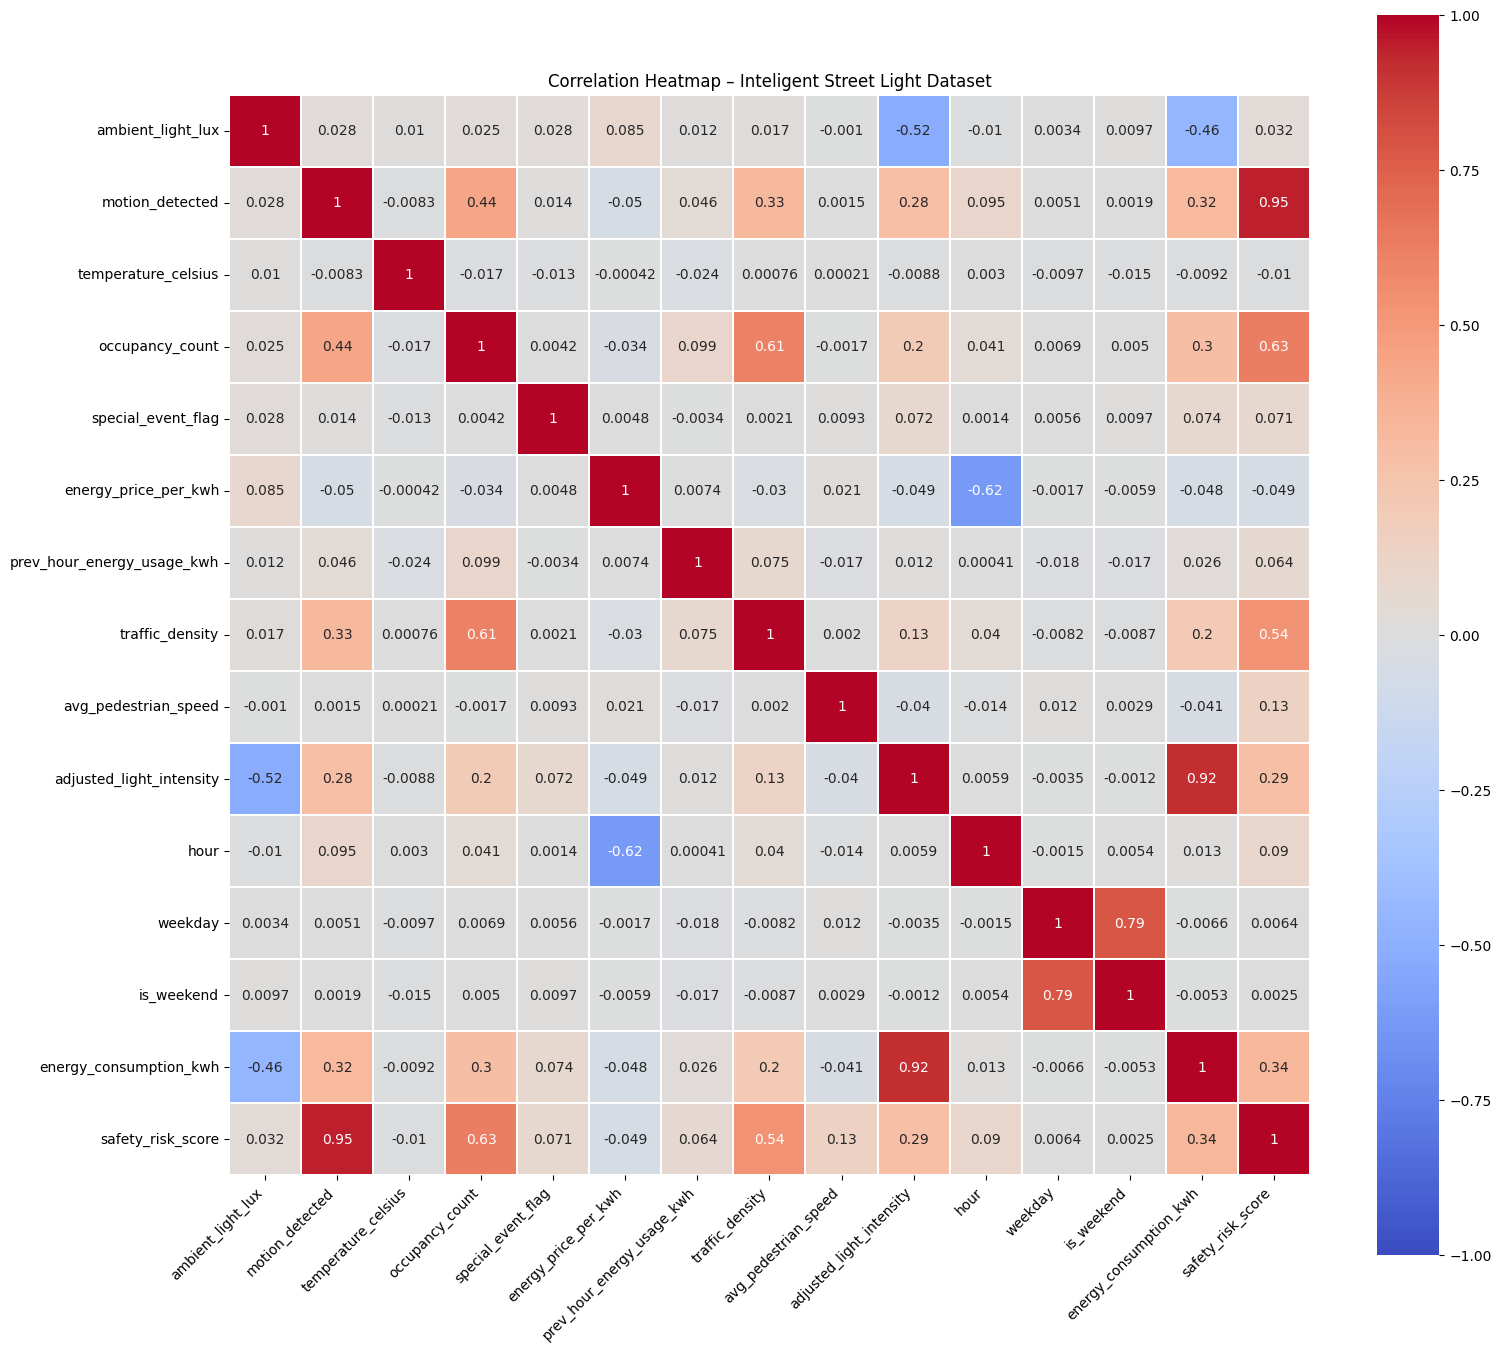
\includegraphics[width=0.4\textwidth]{assets/CorrMatrix.png}
\caption{Correlation heatmap of key numerical features in the smart lighting dataset, highlighting relationships between ambient light, occupancy count, motion detection, and energy usage.}
\label{fig:heatmap}
\end{figure}

\begin{figure}[H]
\centering
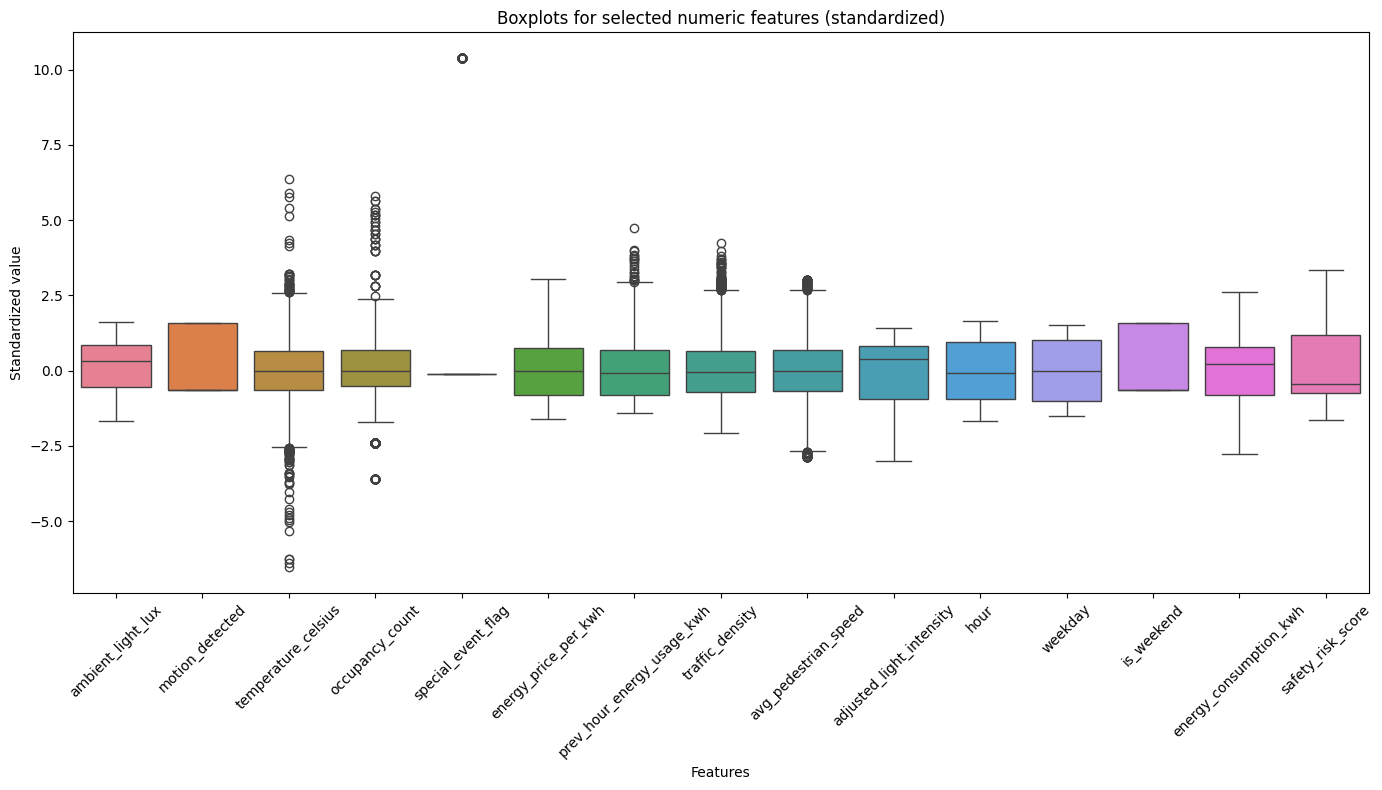
\includegraphics[width=0.45\textwidth]{assets/Boxplot.png}
\caption{Boxplots of key features showing distribution, median, quartiles, and outliers for variables such as ambient light and occupancy count. Outliers indicate potential needs for feature transformation.}
\label{fig:boxplot}
\end{figure}

\section{Model Results and Interpretation}
\subsection{ML Predictor Performance}

This subsection evaluates the predictive performance of the machine learning (ML) model used to estimate adjusted street lighting intensity from contextual and activity-related features. The objective of this analysis is twofold: first, to identify an optimization strategy that yields accurate and stable regression performance; and second, to establish a reliable baseline predictor for subsequent integration with the fuzzy-rule-based control layer.

Multiple gradient-based optimization algorithms were investigated during MLP training, including classical stochastic gradient descent variants and modern adaptive optimizers. Model performance was assessed on a held-out test set using standard regression metrics, namely Root Mean Square Error (RMSE), Mean Absolute Error (MAE), and the coefficient of determination ($R^2$). These metrics jointly capture average prediction error magnitude, robustness to outliers, and overall goodness of fit.

To enable a clear and objective comparison, optimizers were ranked primarily according to RMSE, with MAE and $R^2$ used as secondary criteria. This ranking provides insight into the suitability of each optimizer for learning complex, nonlinear relationships in the smart lighting dataset and informs the selection of the baseline ML predictor used in the hybrid control framework.

\begin{table}[H]
\centering
\caption{Ranking of Optimizers Based on Predictive Performance}
\label{tab:optimizer_ranking}
    \begin{tabular}{c|l|c|c|c|c}
        \hline
        \textbf{Rank} & \textbf{Optimizer} & \textbf{RMSE} & \textbf{MAE} & \textbf{$R^2$} & \textbf{Runtime (s)} \\
        \hline
        1 & Adam      & \textbf{8.174} & 6.472 & \textbf{0.8672} & 94.47 \\
        2 & Nadam     & 8.176 & \textbf{6.456} & 0.8672 & 97.01 \\
        3 & Momentum  & 8.289 & 6.580 & 0.8635 & 79.79 \\
        4 & RMSprop   & 8.289 & 6.523 & 0.8635 & 86.30 \\
        5 & SGD       & 8.312 & 6.595 & 0.8627 & 173.58 \\
        6 & Lion      & 8.419 & 6.649 & 0.8592 & 80.62 \\
        7 & AMSGrad   & 8.549 & 6.750 & 0.8548 & 117.94 \\
        8 & Adagrad   & 61.638 & 58.181 & -6.5491 & 83.78 \\
        9 & Adadelta  & 67.047 & 63.395 & -7.9322 & 101.94 \\
        \hline
    \end{tabular}
\end{table}

Optimizers were ranked according to predictive performance using RMSE as the primary criterion, 
with MAE and $R^2$ used as secondary tie-breakers. Adam achieved the best overall performance, 
closely followed by Nadam, indicating the effectiveness of adaptive moment-based optimization 
for this regression task. Momentum and RMSprop formed a second tier with comparable accuracy.

SGD exhibited slightly inferior performance and substantially longer runtime, while Lion and 
AMSGrad showed moderate degradation in accuracy. Adagrad and Adadelta performed poorly, 
with negative $R^2$ values, indicating divergence and failure to model the target relationship.

\begin{table}[H]
\centering
\caption{Ranking of Regression Models Based on Predictive Performance}
\label{tab:model_ranking}
\begin{tabular}{c|l|c|c|c|c}
\hline
\textbf{Rank} & \textbf{Model} & \textbf{RMSE} & \textbf{MAE} & \textbf{$R^2$} & \textbf{Runtime (s)} \\
\hline
1 & Gradient Boosting & \textbf{$7.2352$} & \textbf{$5.5802$} & \textbf{$0.8960$} & $8.98$ \\
2 & XGBoost & $7.2540$ & $5.6142$ & $0.8954$ & $0.40$\\
3 & Random Forest & $7.2619$ & $5.5807$ & $0.8952$ & $13.73$\\
4 & MLP (Adam) & $8.1738$ & $6.4718$ & $0.8672$ & $94.47$ \\
5 & Ridge Regression & $8.3420$ & $6.6259$ & $0.8617$ & $0.004$\\
6 & Elastic Net & $8.3474$ & $6.6333$ & $0.8615$ & $0.05$\\
7 & Lasso Regression & $8.3482$ & $6.6333$ & $0.8615$ & $0.08$\\
\hline
\end{tabular}
\end{table}

Models were ranked according to predictive accuracy using RMSE as the primary criterion, 
with MAE and $R^2$ used as secondary measures. Gradient Boosting achieved the best overall 
performance, closely followed by XGBoost and Random Forest, confirming the effectiveness 
of ensemble-based methods for capturing nonlinear relationships in the smart lighting data.

The MLP model ranked fourth, outperforming all linear baselines but underperforming 
tree-based ensembles. Despite this, the MLP was selected as the core predictive component 
for the hybrid controller due to its smooth output behavior and compatibility with the 
fuzzy-rule-based correction mechanism. Linear models ranked lowest, reflecting their 
limited capacity to model complex interactions in the dataset.

\subsection{Final Comparison: Standalone MLP vs. Hybrid MLP+Fuzzy Model}

This subsection presents the final comparison between the standalone Multi-Layer Perceptron (MLP) predictor and the hybrid MLP+Fuzzy control model. The objective of this comparison is to differentiate predictive accuracy from control robustness and to assess the effect of incorporating a fuzzy-rule-based correction layer on overall system performance.

\begin{table}[H]
\centering
\caption{Final Performance Comparison of MLP and Hybrid MLP+Fuzzy Models}
\label{tab:final_comparison}
    \begin{tabular}{c|l|c|c|c}
        \hline
        \textbf{Rank} & \textbf{Model} & \textbf{RMSE} & \textbf{MAE} & \textbf{$R^2$} \\
        \hline
        1 & MLP (Adam) & 8.174 & \textbf{6.456} & \textbf{0.8672} \\
        2 & MLP + Fuzzy & \textbf{8.162} & 6.472 & 0.858 \\
        \hline
    \end{tabular}
\end{table}

The standalone MLP achieved the highest predictive accuracy, with an RMSE of 8.174, an MAE of 6.456, and an $R^2$ of 0.8672. Based on these metrics, the MLP ranks first when models are evaluated solely on regression performance. These results confirm the neural network’s ability to capture complex nonlinear relationships between environmental conditions, activity levels, and lighting demand.

The hybrid MLP+Fuzzy model showed a slightly different performance profile, with an RMSE of 8.162, an MAE of 6.472, and an $R^2$ of 0.858, ranking second in predictive accuracy. This minor reduction in accuracy is expected, as the fuzzy layer deliberately adjusts MLP outputs when predictions deviate from rule-based expectations.

Crucially, the hybrid model is not intended to surpass the MLP purely in terms of error minimization. Its design emphasizes robustness, interpretability, and safety-aware decision-making under uncertainty. By constraining extreme or potentially unsafe predictions, the fuzzy layer enforces conservative lighting adjustments in conditions of poor visibility or abnormal activity. Consequently, the hybrid approach accepts a slight loss in predictive accuracy in exchange for enhanced control reliability, making it more suitable for real-world deployment in street lighting systems where safety and explainability are essential.

\section{Results}

The performance of the hybrid EA+MLP+Fuzzy street lighting control system was evaluated in terms of energy efficiency and safety. The system was compared against a baseline scenario using only raw sensor data for lighting decisions.

\subsection{Energy Efficiency}

\begin{figure}[H]
    \centering
    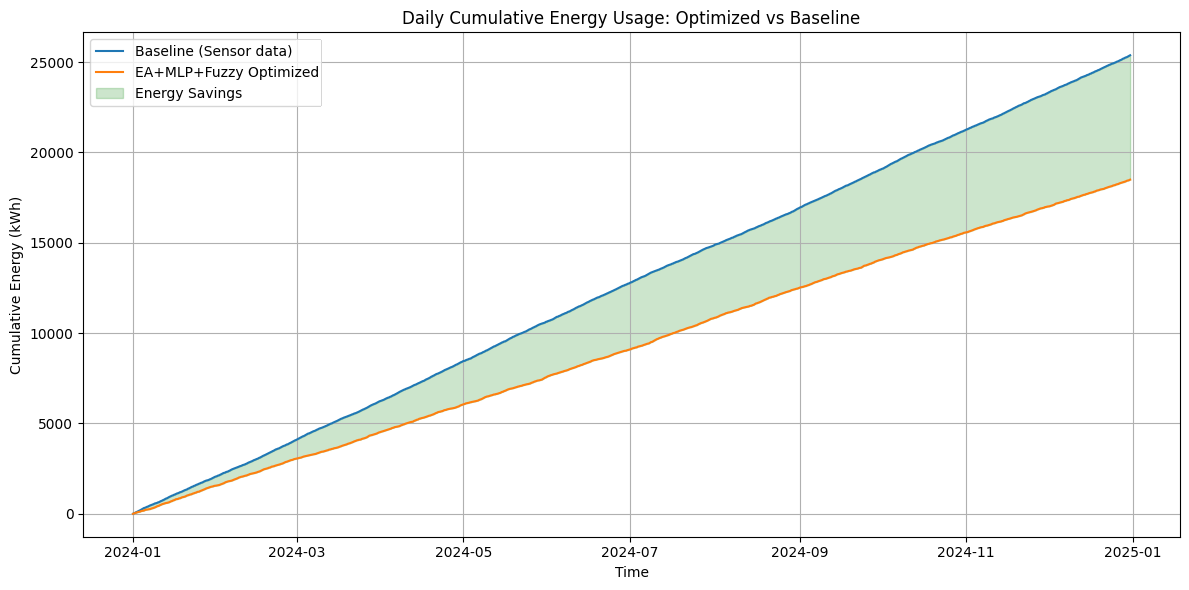
\includegraphics[width=\linewidth]{assets/Results1.png}
    \caption{Daily Cumulative Energy Usage Optimized vs Baseline (Sensor Data)}
    \label{fig:cumulative_energy}
\end{figure}

\begin{figure}[H]
    \centering
    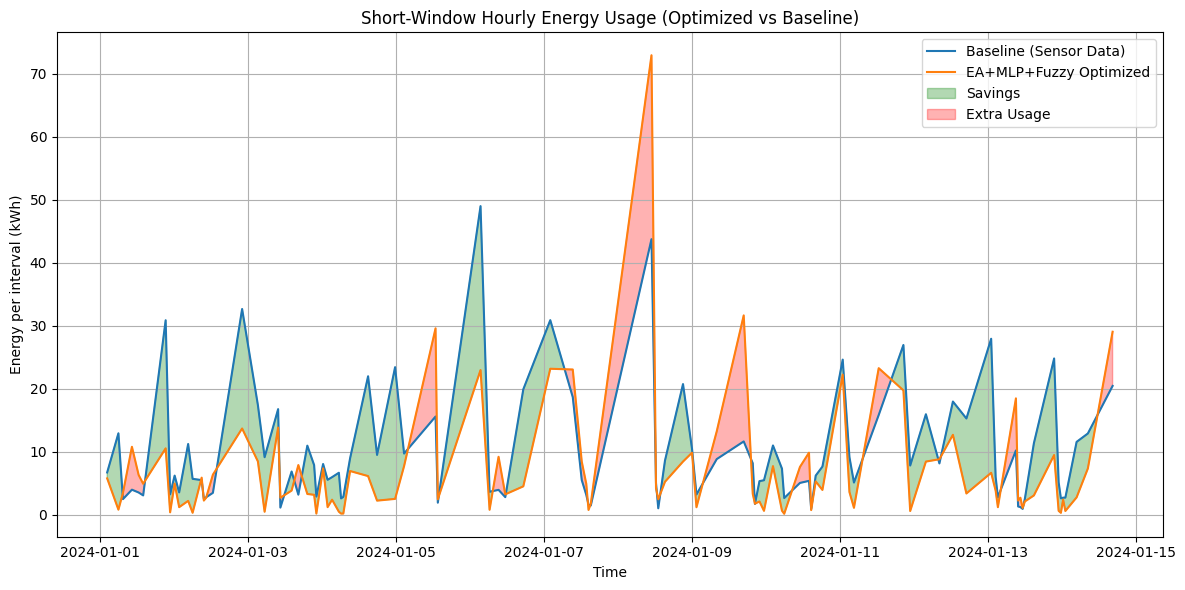
\includegraphics[width=\linewidth]{assets/Results2.png}
    \caption{Short-window hourly energy consumption comparing baseline sensor-driven lighting and EA+MLP+Fuzzy optimized lighting. Green shading indicates energy savings, red indicates slightly higher usage.}
    \label{fig:energy_window}
\end{figure}

Figures~\ref{fig:cumulative_energy} and~\ref{fig:energy_window} illustrate the comparative energy performance of the baseline system driven by raw sensor data and the proposed EA--MLP--Fuzzy optimized strategy at both cumulative and short-term resolutions. The cumulative daily energy consumption plot (Fig.~\ref{fig:cumulative_energy}) shows a clear and consistent divergence between the two trajectories over the one-year evaluation horizon, with the optimized approach exhibiting substantially lower aggregate energy usage. Based on this long-term behavior, the proposed method achieves an average energy saving of \textbf{17.8\%}, demonstrating the effectiveness and stability of the optimization framework. In contrast, the short-window hourly energy usage plot (Fig.~\ref{fig:energy_window}) captures the system behavior at a finer temporal scale. Although the optimized strategy generally operates below the baseline, indicating effective demand reduction, occasional short-lived peaks of higher consumption are observed, which can be attributed to transient control actions or load-balancing adjustments. Nevertheless, these localized increases are outweighed by more frequent and pronounced reductions, as evidenced by the dominant savings regions. Overall, the results confirm that the EA--MLP--Fuzzy approach provides significant long-term energy savings while maintaining robust performance under highly variable operating conditions.

\subsection{Safety Assessment}

\begin{figure}[H]
    \centering
    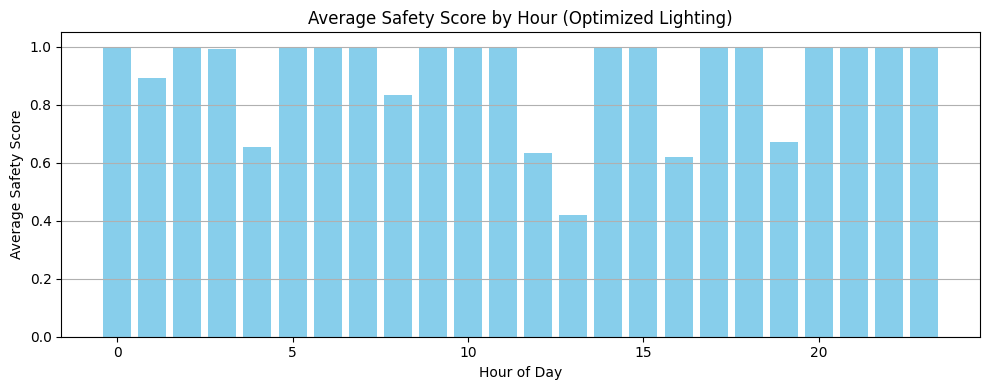
\includegraphics[width=\linewidth]{assets/SafetyPerHourOptimized.png}
    \caption{Average hourly safety score for the optimized lighting system. Shows how safety is maintained across different hours of the day.}
    \label{fig:hourly_safety}
\end{figure}

Safety performance was evaluated using a custom safety score that incorporates environmental visibility and optimized light intensity. Figure~\ref{fig:hourly_safety} presents the average safety score by hour of day for the optimized system. This visualization allows examination of how lighting adjustments maintain safety throughout the daily cycle.

\begin{figure}[H]
    \centering
    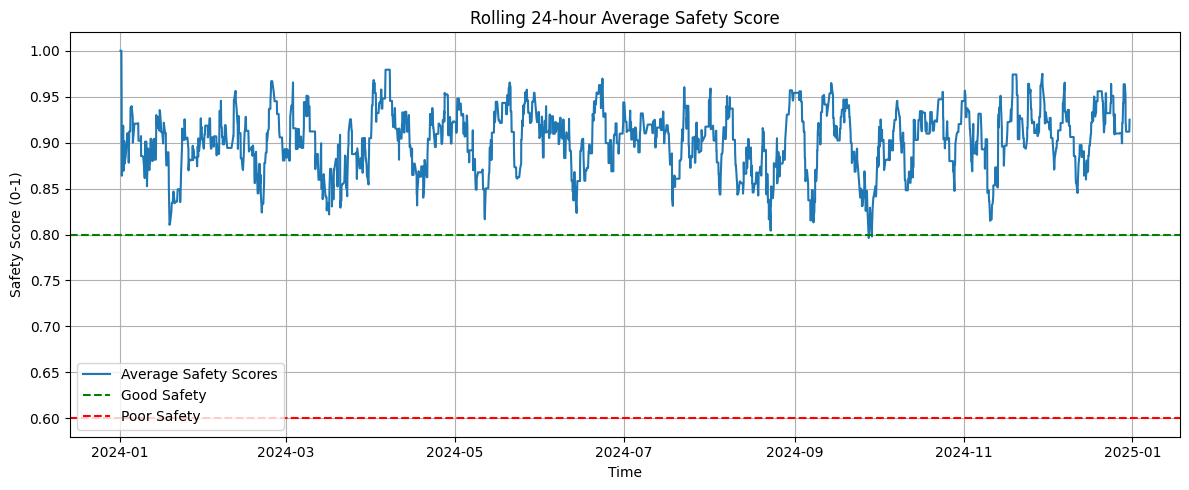
\includegraphics[width=\linewidth]{assets/SafetyScoreInTimeWindow.png}
    \caption{Rolling 24-hour average safety score for the optimized system. Horizontal lines indicate “good” and “poor” safety thresholds.}
    \label{fig:rolling_safety}
\end{figure}

Figure~\ref{fig:rolling_safety} shows the rolling 24-hour average safety score. Horizontal reference lines indicate thresholds for “good” (0.8) and “poor” (0.6) safety levels. The rolling average provides a clearer picture of how safety is maintained over time and highlights periods where intervention may be needed.

\subsection{Limitations and Future Work}
The study’s limitations include:

\begin{itemize}
\item Use of a synthetic or limited dataset, which may not fully capture real-world variability.
\item Manual fuzzy rule design, which may not be globally optimal.
\item Proxy safety metrics instead of field-measured incidents.
\end{itemize}

Future work could address these limitations by:

\begin{itemize}
\item Incorporating real-world sensor data.
\item Automating fuzzy rule and membership tuning via evolutionary algorithms or optimization frameworks.
\item Extending the system to integrate city-wide coordination or multi-objective optimization (energy, safety, comfort).
\end{itemize}

\section{Conclusion}

This work presented a comprehensive study of a smart street lighting control system based on a hybrid combination of machine learning and classical artificial intelligence methods. The proposed approach integrates a data-driven predictor for short-term pedestrian activity with a fuzzy-rule-based expert layer that translates predictions and contextual information into interpretable lighting decisions.

The results indicate that adaptive lighting strategies can substantially reduce unnecessary energy consumption compared to static schedules, particularly during low-demand periods. At the same time, the fuzzy expert layer enforces conservative behavior under uncertain or adverse conditions, ensuring that safety and visibility requirements are maintained. This balance between efficiency and safety is a key strength of the hybrid architecture.

Beyond quantitative performance metrics, the proposed system emphasizes transparency, robustness, and practical deployability. Interpretability through fuzzy rules supports accountability and facilitates integration with regulatory constraints. Its modular design enables scalability across urban areas and resilience to partial system failures. Ethical, privacy, and sustainability considerations further highlight the broader implications of deploying adaptive control in public infrastructure.

Overall, the study demonstrates that hybrid AI approaches offer a promising pathway for intelligent and responsible smart city applications. By combining predictive power with human-understandable reasoning, adaptive street lighting systems can meaningfully contribute to energy efficiency, public safety, and long-term urban sustainability.

\bibliographystyle{IEEEtran}
\bibliography{references}
\bibitem{smartlighting_dataset}
IoT-Enabled Smart Lighting Dataset, Kaggle.
[Online]. Available: \url{https://www.kaggle.com/datasets/ziya07/iot-enabled-smart-lighting-dataset}.
Accessed: Jan. 14, 2026.

\bibitem{zadeh1965fuzzy}
L. A. Zadeh, ``Fuzzy sets,'' \emph{Information and Control}, vol. 8, no. 3, pp. 338--353, 1965.

\bibitem{ross2010fuzzy}
T. J. Ross, \emph{Fuzzy Logic with Engineering Applications}, 3rd ed.
Hoboken, NJ, USA: Wiley, 2010.

\bibitem{holland1992genetic}
J. H. Holland, ``Genetic algorithms,'' \emph{Scientific American},
vol. 267, no. 1, pp. 66--73, 1992.

\bibitem{kingma2015adam}
D. P. Kingma and J. Ba, ``Adam: A method for stochastic optimization,''
in \emph{Proc. Int. Conf. Learn. Representations (ICLR)}, 2015.

\bibitem{wilcoxon1945individual}
F. Wilcoxon, ``Individual comparisons by ranking methods,''
\emph{Biometrics Bulletin}, vol. 1, no. 6, pp. 80--83, 1945.

\bibitem{molina2018smartlighting}
M. Molina \emph{et al.}, ``Smart street lighting systems using machine learning techniques,''
\emph{IEEE Trans. Intell. Transp. Syst.}, vol. 19, no. 5, pp. 1421--1430, May 2018.


\end{document}
